\documentclass{beamer}
\usepackage[utf8]{inputenc}
\usepackage[T1]{fontenc}
\usepackage{lmodern}
\usepackage{amsmath}
\usepackage{tikz}
\usepackage{xcolor} % Farben
\usepackage{fancyvrb} % Code
\usepackage[absolute,overlay]{textpos} % Bilder irgendwohin
\usepackage{bm} % Fett in Mathemodus
\usepackage{siunitx} % Einheiten
\usepackage{multicol} % Equations nebeneinander
\usepackage{algorithm2e} % Algorithmen
\usepackage{array} % Tabellenspalten zentriert
\usepackage{hyperref} % Links

\usecolortheme{seahorse}
\definecolor{dark}{rgb}{0, 0.1, 0.3}
\definecolor{light}{rgb}{0.9, 0.933, 1}
\setbeamercolor{normal text}{fg=black}
\setbeamercolor{structure}{fg=dark}
\setbeamercolor{footline}{fg=black}
\setbeamercolor{frametitle}{fg=light,bg=dark}
\setbeamertemplate{itemize items}[circle]
\beamertemplatenavigationsymbolsempty
\addtobeamertemplate{navigation symbols}{}{
    \usebeamerfont{footline}
    \usebeamercolor[fg]{footline}
    {\footnotesize \insertframenumber\\\vspace{0.15cm}}
}
\setbeamertemplate{title page}{
    \begin{center}
    Projektgruppe FastSense\\\vspace{1cm}
    \begin{LARGE}
    Meilenstein 2\\\vspace{0.5cm}   
    Hardware Accelerated TSDF SLAM
    \end{LARGE}\\\vspace{1cm}
    28. Oktober 2020
    \end{center}
}

\begin{document}

{\setbeamertemplate{navigation symbols}{}
\begin{frame}
\titlepage
\end{frame}}

\begin{frame}
\frametitle{Inhalt}
\tableofcontents
\end{frame}



\section{Ziele und Anforderungen}
\begin{frame}{}
\begin{center}
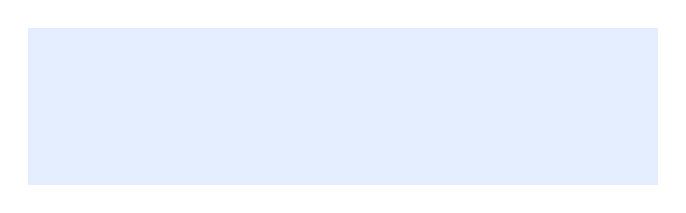
\begin{tikzpicture}
\fill[light] (0, 0) rectangle (8, 2);
\node[dark] at (4, 1) {\begin{LARGE}\secname\end{LARGE}};
\end{tikzpicture}
\end{center}
\end{frame}

\subsection{Ziele für MS2}
\begin{frame}{\subsecname}
\begin{itemize}
    \item Implementation von inkrementellem SLAM mit TSDF in "autarker" Box
    \item Vorimplementation in Software
    \item Implementation von Bottleneck-Komponenten in Hardware
    \item Speicherung von Pose-Graph und TSDF-Karte zur Rekonstruktion des kompletten explorierten Bereichs
    \item Evaluation durch Zeit- und Strommessung
\end{itemize}
\end{frame}

\subsection{Funktionale Anforderungen}
\begin{frame}{\subsecname}
\begin{itemize}
\item{Lokale TSDF-Map ausgeben}
\item{Aktuelle 6D-Pose ausgeben}
\item{Map auf Basis der IMU und Velodyne-Daten}
\item{Trajektorie und TDSF-Map für jede Pose speichern}
\item{Parameter zur Laufzeit anpassbar}
\end{itemize}
\end{frame}

\subsection{Nicht-Funktionale Anforderungen}
\begin{frame}{\subsecname}
\begin{itemize}
\item{HW-Plattform: Trenz-Board, SW-Plattform: Vitis}
\item{FPGA-Beschleunigung der Algorithmen}
\item{Sensoren direkt am Board}
\item{Unit-Tests}
\item{Testbench}
\begin{itemize}
\item{Integration, Strommessung, Zeitmessung, Visualisierung}
\end{itemize}
\item{Logging}
\end{itemize}
\end{frame}



\section{Hauptspeise}
\begin{frame}{}
\begin{center}
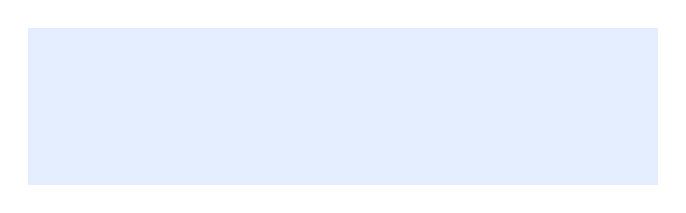
\begin{tikzpicture}
\fill[light] (0, 0) rectangle (8, 2);
\node[dark] at (4, 1) {\begin{LARGE}\secname\end{LARGE}};
\end{tikzpicture}
\end{center}
\end{frame}

\subsection{Algorithmus}
\begin{frame}{\subsecname}
TODO: gute visuelle Darstellung, möglichst kein unnötiger Text
\begin{center}
\begin{tikzpicture}
\draw (0, 0) rectangle +(2, 2);
\draw [->] (2, 1) -- (4, 1);
\draw (4, 0) rectangle +(2, 2);
\end{tikzpicture}
\end{center}
\end{frame}

\subsection{Recap: Prototyping Demo}
\begin{frame}{\subsecname}
\begin{itemize}
    \item Registrierung mithilfe von IMU
    \item Gute Parameterkombination herausgefunden
    \item Geplante Funktionalität war vorhanden und in RViz darstellbar
    \item Erkannte Probleme / Bottlenecks:
    \begin{itemize}
        \item Laufzeit stark abhängig von der Auflösung der Karte
        \item Probleme mit Orientierung (kurz nach Demo gefixt)
        \item Insgesamt noch recht langsam ($\sim$0.5s/Scan auf Glumanda, 2-5s/Scan in Testwelt)
        \item Bottlenecks Registrierung und TSDF-Update (dachten wir)
    \end{itemize}
\end{itemize}
\end{frame}

\subsection{Hardware Implementierung}
\begin{frame}{\subsecname}
TODO: infos zu reg und tsdf, wie visuell darstellen?
\end{frame}

\subsection{FastSense Prototyp}
\begin{frame}{\subsecname}
\begin{center}
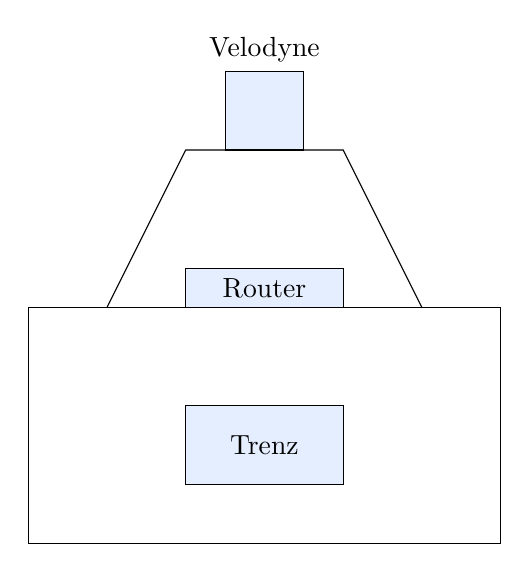
\begin{tikzpicture}
\draw (0, 0) rectangle (6, 3);
\draw (1, 3) -- (2, 5) -- (4, 5) -- (5, 3);
\draw [fill=light] (2, 0.75) rectangle +(2, 1);
\node at (3, 1.25) {Trenz};
\draw [fill=light] (2, 3) rectangle +(2, 0.5);
\node at (3, 3.25) {Router};
\draw [fill=light] (2.5, 5) rectangle +(1, 1);
\node [above] at (3, 6) {Velodyne};
\end{tikzpicture}
\end{center}
\end{frame}

\begin{frame}{\subsecname}
\begin{center}
\begin{tabular}{cc}
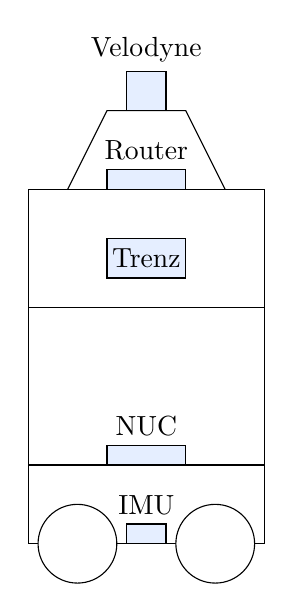
\begin{tikzpicture}[scale=0.5]
\draw (0, 0) rectangle (6, 3);
\draw (1, 3) -- (2, 5) -- (4, 5) -- (5, 3);
\draw [fill=light] (2, 0.75) rectangle +(2, 1);
\node at (3, 1.25) {Trenz};
\draw [fill=light] (2, 3) rectangle +(2, 0.5);
\node [above] at (3, 3.5) {Router};
\draw [fill=light] (2.5, 5) rectangle +(1, 1);
\node [above] at (3, 6) {Velodyne};
\draw (0, 0) -- (0, -6) -- (6, -6) -- (6, 0);
\draw (0, -4) -- (6, -4);
\draw [fill=light] (2, -4) rectangle +(2, 0.5);
\node [above] at (3, -3.5) {NUC};
\draw [fill=light] (2.5, -6) rectangle +(1, 0.5);
\node [above] at (3, -5.5) {IMU};
\draw [fill=white] (1.25, -6) circle (1);
\draw [fill=white] (4.75, -6) circle (1);
\end{tikzpicture} &
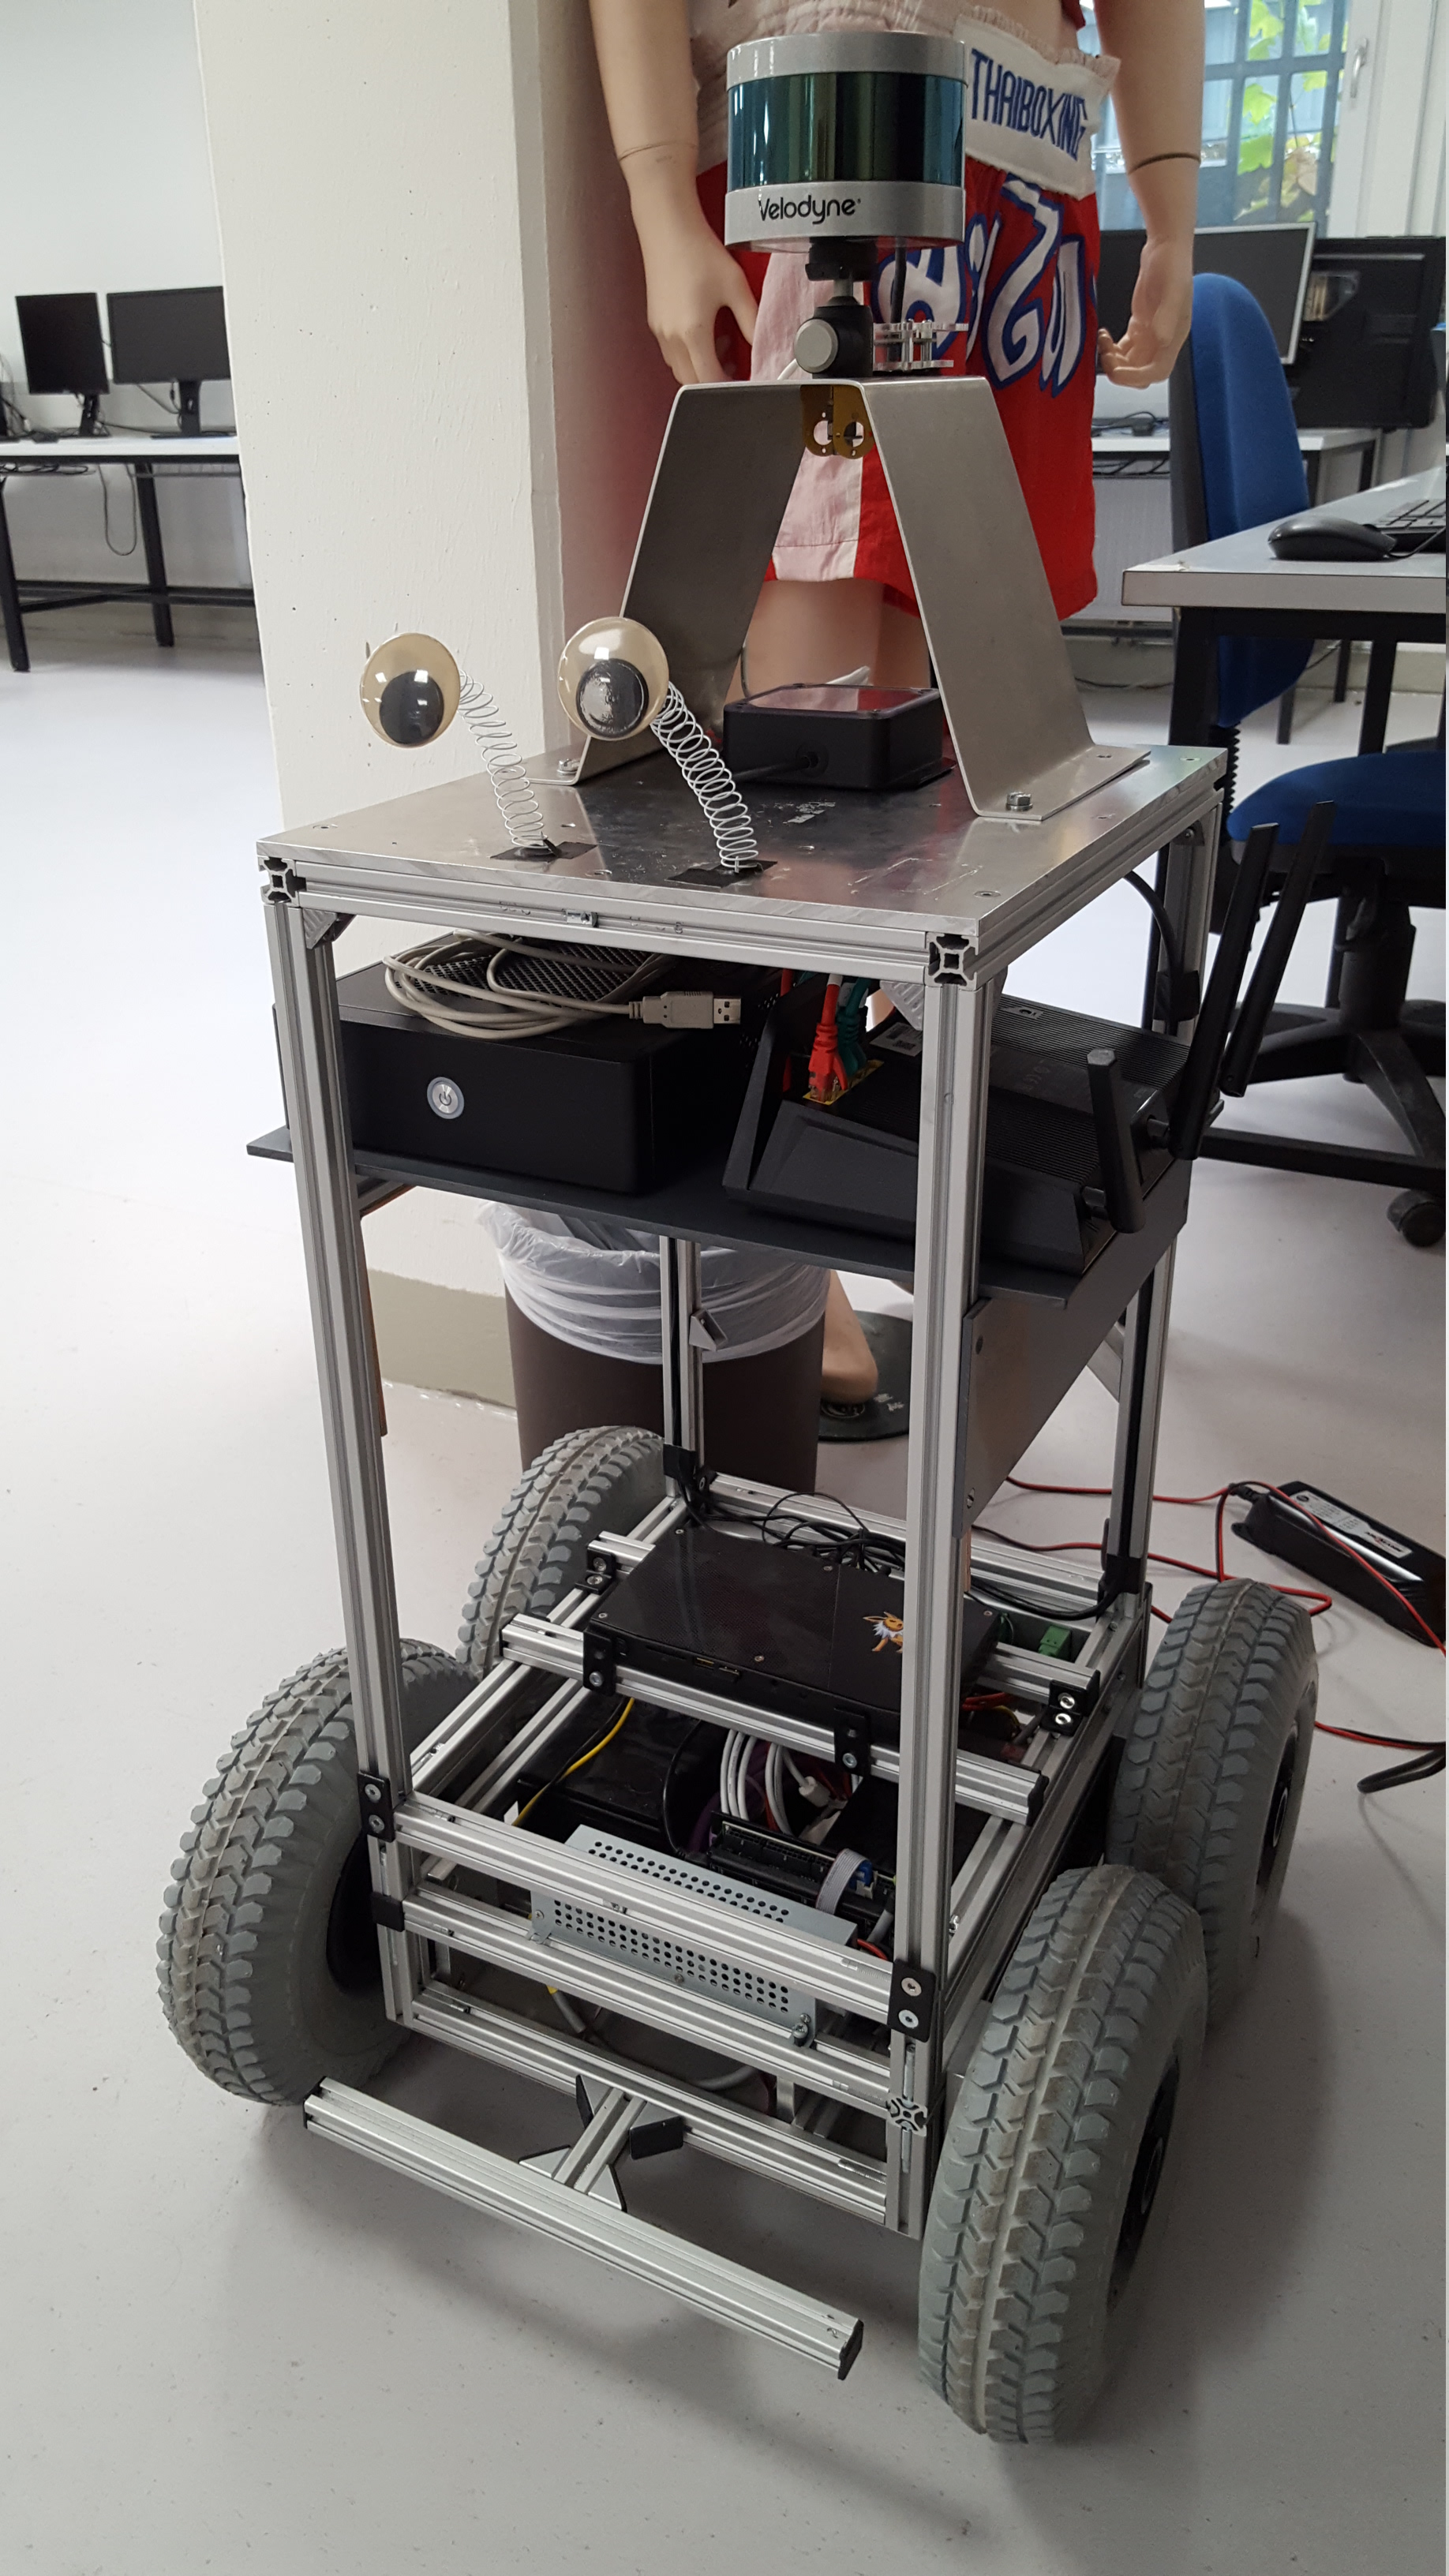
\includegraphics[height=8cm]{images/robot.jpg}
\end{tabular}
\end{center}
\end{frame}

\subsection{Kommunikation}
\begin{frame}{\subsecname}
TODO: Kommunikation von Julian
\end{frame}



\section{Evaluation}
\begin{frame}{}
\begin{center}
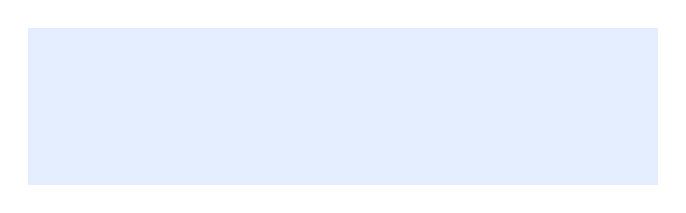
\begin{tikzpicture}
\fill[light] (0, 0) rectangle (8, 2);
\node[dark] at (4, 1) {\begin{LARGE}\secname\end{LARGE}};
\end{tikzpicture}
\end{center}
\end{frame}

\subsection{Strom}
\begin{frame}{\subsecname}
\begin{center}
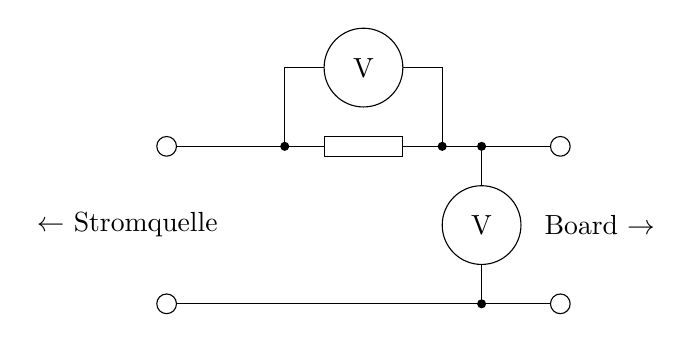
\begin{tikzpicture}[scale=0.5]
\draw (0, 0) circle (0.25);
\draw (0, 4) circle (0.25);
\draw (10, 0) circle (0.25);
\draw (10, 4) circle (0.25);
\draw (0.25, 0) -- (9.75, 0);
\draw (0.25, 4) -- (9.75, 4);
\draw (3, 4) -- (3, 6) -- (7, 6) -- (7, 4);
\draw (8, 0) -- (8, 4);
\draw [fill=black] (3, 4) circle (0.1);
\draw [fill=black] (7, 4) circle (0.1);
\draw [fill=black] (8, 0) circle (0.1);
\draw [fill=black] (8, 4) circle (0.1);
\draw [fill=white] (5, 6) circle (1) node{V};
\draw [fill=white] (8, 2) circle (1) node{V};
\draw [fill=white] (4, 3.75) rectangle (6, 4.25);
\node at (-1, 2) {$\leftarrow$ Stromquelle};
\node at (11, 2) {Board $\rightarrow$};
\end{tikzpicture}
\end{center}
\end{frame}

\begin{frame}{\subsecname}
TODO: Ergebnisse
\end{frame}

\subsection{Zeit}
\begin{frame}{\subsecname}
\centering
\begin{tabular}{ |p{3cm}||p{2cm}|p{2cm}|p{2cm}|  }
 \hline
 \multicolumn{4}{|c|}{Zeitmessung (ms)} \\
 \hline
 Abschnitt      & Durchschnitt & Min & Max\\
 \hline
 Preprocessing  &          ??? & ??? & ??? \\
 Registrierung  &          ??? & ??? & ??? \\
 TSDF Update    &          ??? & ??? & ??? \\
 Map Shift      &          ??? & ??? & ??? \\
 \hline
\end{tabular}
\end{frame}

\begin{frame}{\subsecname}
\centering
\begin{tabular}{ |l||l|l|  }
 \hline
 \multicolumn{3}{|c|}{Vergleich Vitis -- Realität} \\
 \hline
 Abschnitt      & Vitis & Gemessen\\
 \hline
 Registrierung  & 0.9ms $\cdot$ 100 = 90ms & ??? \\
 TSDF Update    & 477ms & ??? \\
 \hline
\end{tabular}
\end{frame}

\begin{frame}{\subsecname}
\centering
\begin{tabular}{ |p{3cm}||p{2cm}|p{2cm}|p{2cm}|  }
 \hline
 \multicolumn{4}{|c|}{Vergleich (Durchschnitt, ms)} \\
 \hline
 Programm       & FastSense & Prototyp & Prototyp \\
 \hline
 System         &     Board &    Board &      NUC \\
 \hline
 Preprocessing  &       ??? &      ??? &      ??? \\
 Registrierung  &       ??? &      ??? &      ??? \\
 TSDF Update    &       ??? &      ??? &      ??? \\
 Map Shift      &       ??? &      ??? &      ??? \\
\hline
\end{tabular}
\end{frame}



\section{Fazit}
\begin{frame}{}
\begin{center}
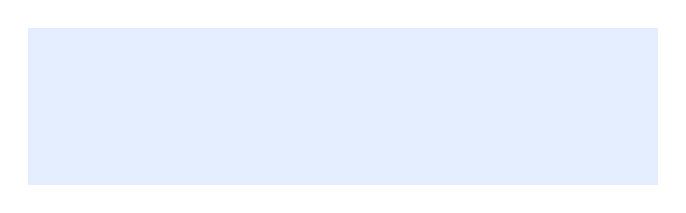
\begin{tikzpicture}
\fill[light] (0, 0) rectangle (8, 2);
\node[dark] at (4, 1) {\begin{LARGE}\secname\end{LARGE}};
\end{tikzpicture}
\end{center}
\end{frame}

\subsection{Bisherige Verbesserungen}
\begin{frame}{\subsecname}
\begin{itemize}
\item{Registrierung}
\begin{itemize}
\item{Auslagerung von Point to TSDF auf Hardware}
\item{Auslagerung von Pointcloud Transformation auf Hardware}
\end{itemize}
\item{TSDF}
\end{itemize}
\end{frame}

\subsection{Verbesserungspotenzial}
\begin{frame}{\subsecname}
\begin{itemize}
\item{Registrierung}
\begin{itemize}
\item{Drift entfernen (aktuell noch leichter Drift (1cm/s) in alle 3 Richtungen)}
\item{Komplett in Hardware (Overhead ist fast dreimal so hoch wie der eigentliche Aufruf)}
\end{itemize}
\end{itemize}
\end{frame}

\subsection{Projektmanagement}
\begin{frame}{\subsecname}
\begin{textblock*}{12.7cm}(0cm,1cm)
\begin{center}
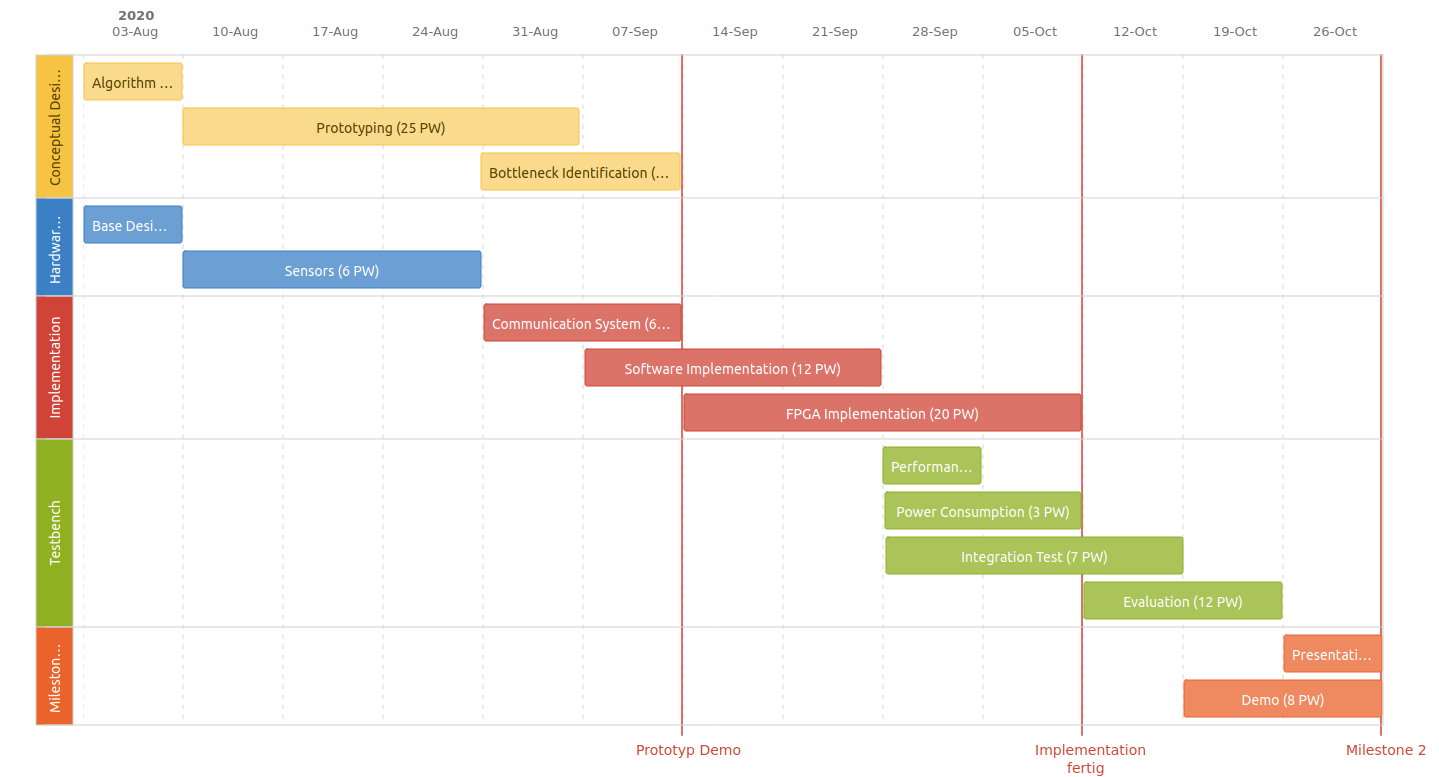
\includegraphics[height=6.9cm]{images/roadmap.png}
\end{center}
\end{textblock*}
\end{frame}

\begin{frame}{\subsecname}
\begin{textblock*}{12.7cm}(0cm,1cm)
\begin{center}
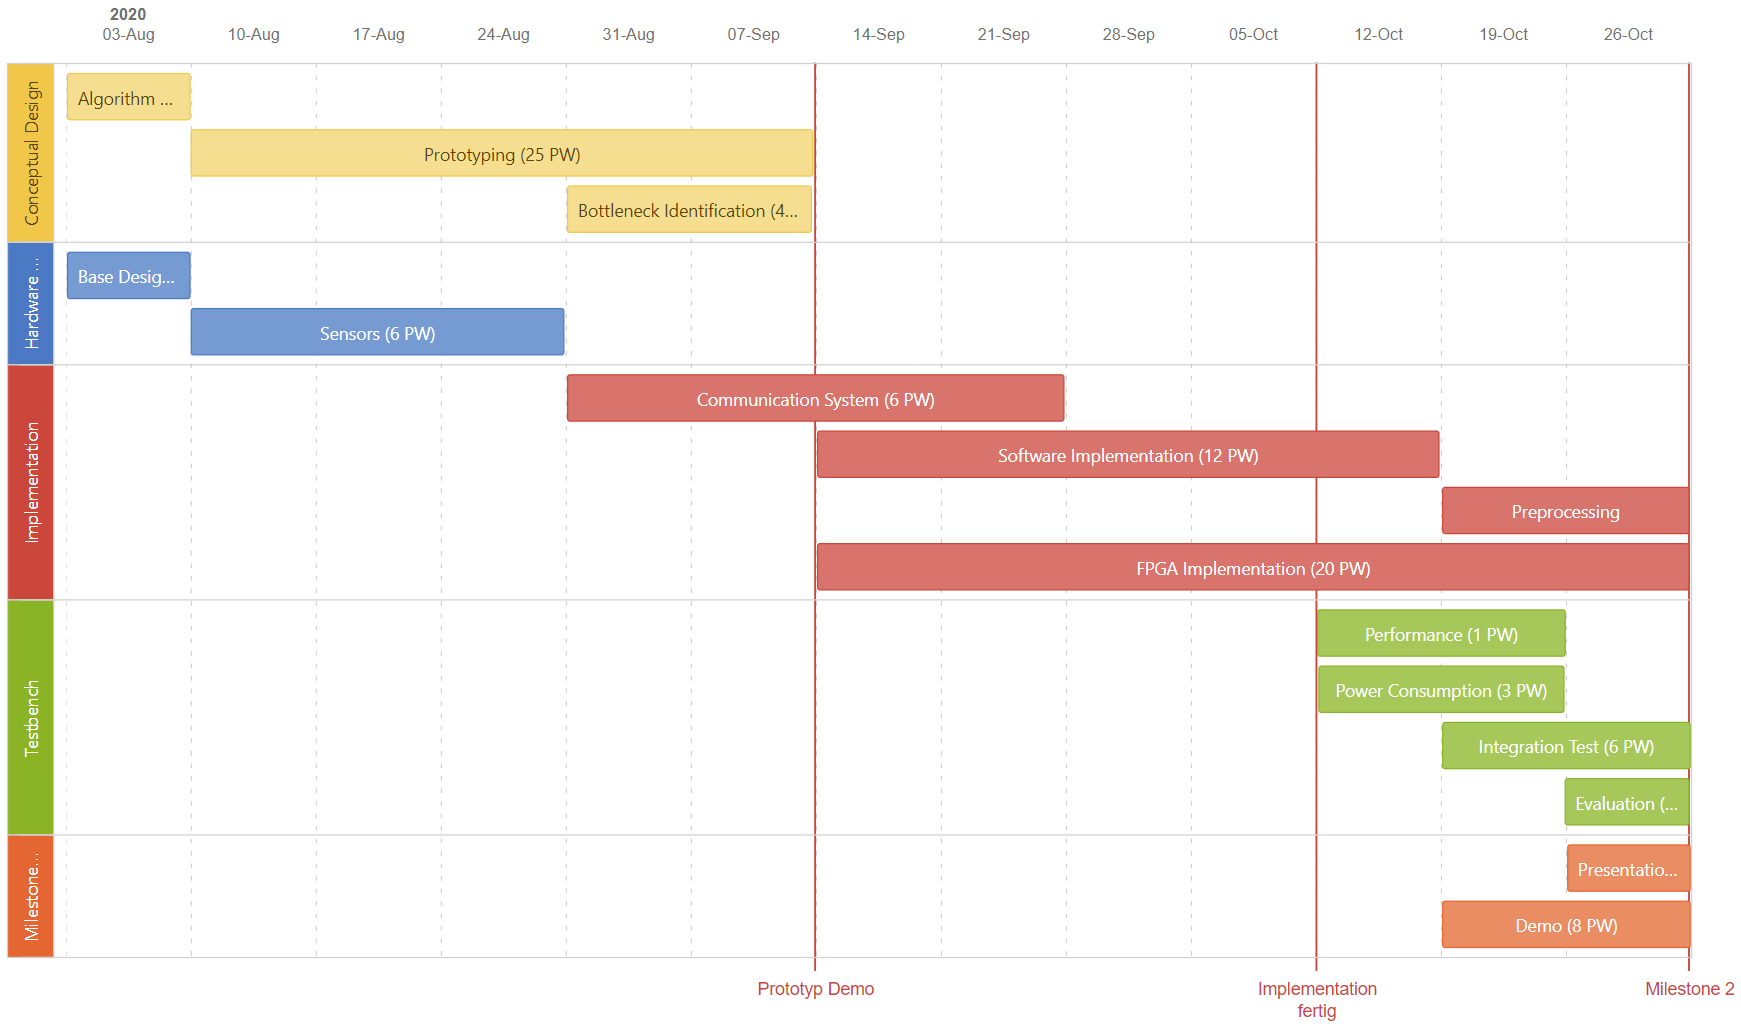
\includegraphics[height=7.3cm]{images/roadmap_new.png}
\end{center}
\end{textblock*}
\end{frame}

\section{Ausblick / MS3}
\begin{frame}{\secname}
\begin{itemize}
\item{Aufbau einer SLAM-Box mittels CAD}
\begin{itemize}
\item{Nutzung als Sensor}
\item{Einfache Portierung zwischen Drohne, Roboter, Rucksack etc.}
\item{Festes Interface, einfache Bedienung, Kapselung}
\end{itemize}
\item{Verbesserung und Optimierung des Algorithmus}
\item{Mesh-Generierung auf Basis der TSDF Werte}
\item{Loop Closing}
\item{???}
\end{itemize}
TODO: Mehr Ideen für MS3?
\end{frame}

\end{document}
